\chapter{The Menu Bar}

The main menu bar\index{menu bar} at the top of the OPUS GUI main window has three dropdown
menus: File, Tools, and Help.  The File menu includes the standard
operations of opening a project, saving a project, saving a project under a
new name, closing an OPUS Project, and finally exiting the OPUS GUI\@.  Help
offers an About option which produces a dialog box with information about
OPUS and a set of links to the UrbanSim website, online documentation, and
the GNU License.  The Tools menu provides access to several general tools,
described below.

Most of the items in the main menu bar are accessible from a secondary menu
bar just above the tabs on the left side of the OPUS GUI window.  Hovering
over each icon will yield a tooltip with the item's description.

\section{Tools}

The Tools menu\index{Tools menu}, shown in figure \ref{fig:menu-bar-tools}, enables users to
adjust settings and preferences, as well as opening different tabs in the
right set of tabs.  The items labeled ``Log View'' and ``Result Browser''
will each open new tabs on the right.  The Result Browser is covered in
greater detail in section \ref{sec:interactive-result-exploration}.  The
items labeled ``Variable Library,'' ``Preferences,'' and ``Database
Connection Settings'' each open a popup when clicked.  (On the Macintosh,
the ``Preferences'' item is under ``Python'' rather than ``Tools.'')  The
Variable Library is further discussed in section
\ref{chap:variable-library}.

\begin{figure}[htp]
\begin{center}
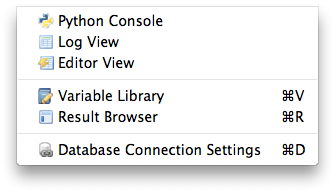
\includegraphics[scale=0.4]{part-gui/images/menu-bar-tools.png}
\end{center}
\caption{Tools Menu}
\label{fig:menu-bar-tools}
\end{figure}


\section{Preferences}

The Preferences dialog box\index{Preferences dialog box} changes some user interface related options in
the OPUS UI.  The dialog box is split into two sections, font preferences\index{font preferences}
and previous project preferences\index{previous project preferences}.  The font preferences section allows
users to adjust font sizes specific to different areas of the GUI.  The
previous project preferences section contains a checkbox allowing users to
open the most recently opened project each time OPUS GUI is started, this
is turned off by default.  Changes to the user preferences take effect as
soon as either the ``Apply'' or ``OK'' buttons are clicked.

\section{Database Server Connections}\label{sec:database-server-connections}

Database connections can be configured in the Database Server Connections
dialog launched from the Tools menu.  The Database Server Connections\index{Database Server Connections}
dialog, pictured in Figure \ref{fig:menu-bar-database-connections}, holds
connection information for four database servers.  Each connection is used
for a specific purpose.  While there are four different connections that
must be configured, each may be configured to use the same host.  Every
connection requires a protocol, host name, user name, and password to be
entered.  Editing the protocol field produces a drop down of database
protocols that UrbanSim is able to use.  If a server has been setup for
UrbanSim's use choose the protocol that corresponds to the type of SQL
server being used.  If no SQL server is setup for a particular use, SQLite
may be used.  SQLite will create a local flat-file database\index{flat-file database} instead of a
remote server.  UrbanSim currently supports MySQL, Microsoft SQL Server,
Postgres, and SQLite.

The Database Connection Settings are saved when the Accept Changes button
is pressed, ensuring that all future database connections will be made
using the new settings.  Database connections that are still in use while
the database connection settings are being edited will not be changed until
the connection is reestablished, for this reason it may be necessary to
reopen any open project after changing the database connection settings.

\begin{figure}[htp]
\begin{center}
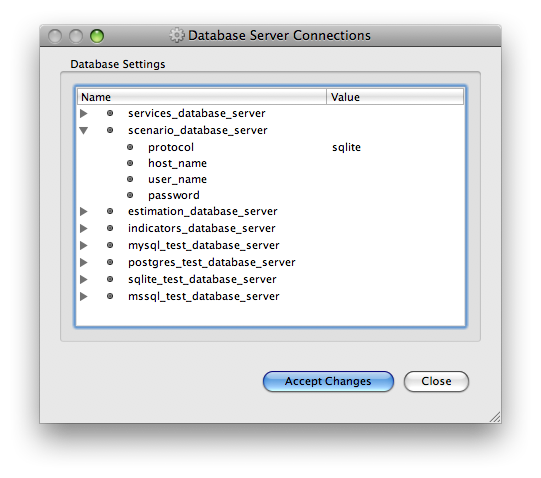
\includegraphics[scale=0.6]{part-gui/images/menu-bar-database-connections.png}
\end{center}
\caption{Database Connections}
\label{fig:menu-bar-database-connections}
\end{figure}
